%%%%%%%%%%%%%%%%%%%%%%%%%%%%%%%%
% Template for 18-845 GP reports
%%%%%%%%%%%%%%%%%%%%%%%%%%%%%%%

\documentclass{sig-alternate-10pt}
\usepackage{auto-pst-pdf}
\usepackage{graphics}
\usepackage{caption}
\usepackage{url}
\usepackage{multirow}

\begin{document}

\title{Comparative Study of Containers and Virtual Machines}
%
% You need the command \numberofauthors to handle the 'placement
% and alignment' of the authors beneath the title.
%
% For aesthetic reasons, we recommend 'three authors at a time'
% i.e. three 'name/affiliation blocks' be placed beneath the title.
%
% NOTE: You are NOT restricted in how many 'rows' of
% "name/affiliations" may appear. We just ask that you restrict
% the number of 'columns' to three.
%
% Because of the available 'opening page real-estate'
% we ask you to refrain from putting more than six authors
% (two rows with three columns) beneath the article title.
% More than six makes the first-page appear very cluttered indeed.
%
% Use the \alignauthor commands to handle the names
% and affiliations for an 'aesthetic maximum' of six authors.
% Add names, affiliations, addresses for
% the seventh etc. author(s) as the argument for the
% \additionalauthors command.
% These 'additional authors' will be output/set for you
% without further effort on your part as the last section in
% the body of your article BEFORE References or any Appendices.

\numberofauthors{1} %  in this sample file, there are a *total*
% of EIGHT authors. SIX appear on the 'first-page' (for formatting
% reasons) and the remaining two appear in the \additionalauthors section.
%
\author{
% You can go ahead and credit any number of authors here,
% e.g. one 'row of three' or two rows (consisting of one row of three
% and a second row of one, two or three).
%
% The command \alignauthor (no curly braces needed) should
% precede each author name, affiliation/snail-mail address and
% e-mail address. Additionally, tag each line of
% affiliation/address with \affaddr, and tag the
% e-mail address with \email.
%
% 1st. author
\alignauthor
Alexander Yu\\
       \affaddr{Carnegie Mellon University}\\
       \email{ayu1@andrew.cmu.edu}
}
% There's nothing stopping you putting the seventh, eighth, etc.
% author on the opening page (as the 'third row') but we ask,
% for aesthetic reasons that you place these 'additional authors'
% in the \additional authors block, viz.
\additionalauthors{Additional authors: John Smith (The Th{\o}rv{\"a}ld Group,
email: {\texttt{jsmith@affiliation.org}}) and Julius P.~Kumquat
(The Kumquat Consortium, email: {\texttt{jpkumquat@consortium.net}}).}
\date{30 July 1999}
% Just remember to make sure that the TOTAL number of authors
% is the number that will appear on the first page PLUS the
% number that will appear in the \additionalauthors section.

\maketitle
\begin{abstract}
This paper presents the efforts made to recreate results from two comparative studies on the performance of containers and virtual machines by Felter et al.\cite{felter:2014} and Sharma et al.\cite{sharma:2016}.

The main contribution of this paper is an evaluation of the performance of containers and VMs in multiple aspects, using a suite of workloads that stress CPU and memory. The paper uses Docker\cite{docker} and VirtualBox\cite{virtualbox} as representative containers and VMs, respectively. The results are consistent with that of the other two studies, demonstrating that the performance of containers is better than VMs in almost all cases and rivals in that of bare-metal environments in most cases as well.
\end{abstract}

\category{C.4}{Performance of Systems}{}
\category{D.2.6}{Software Engineering}{Programming Environments}
\category{D.2.8}{Software Engineering}{Metrics}
\category{D.4.8}{Operating Systems}{Performance}

\terms{Measurement, Performance}

\keywords{Containers, Virtual Machines, Measurement, Performance, Cluster Computing}

\section{Introduction}
Virtualization is now becoming more and more prevalent and important due to the rise and accessibility of data centers and cloud environments. Any regular user is now able to gain the benefits of and/or experiment with different virtualization technologies from various vendors, such as VirtualBox, KVM, Docker, and so on. Virtualized environments are also available via cloud providers. Amazon's EC2 platform is one of the most popular choices and recently switched to using a customized version of KVM for their virtualization needs. The two most popular techniques are operating system virtualization (containers), and hardware virtualization (VMs). There is a large amount of literature evaluating performance in this area, ranging from evaluations of individual implementations of a technique to comparisons between various implementations of a certain technique to comparisons between certain implementations of various techniques. 

Virtualization in general provides various benefits, such as flexible allocation of hardware resources in terms of both how the resources are mapped and how much is mapped, and support for multiple virtualized applications to share a physical server, which is also referred to as multi-tenancy\cite{sharma:2016}. Hardware virtualization has been the dominant virtualization technology for a long time but operating system (OS) or container-based virtualization has experienced a renaissance in popularity in recent years, especially with the rise of Docker. 

This paper focuses on attempting to recreate the results published by two papers comparing specific container and VM implementations. VirtualBox and Docker are used as the representative VM and container technologies, respectively, because of their accessibility and ease of use. This makes them more probable choices for most users. As such, the main goal is to determine if the papers' results are still accurate with different container and VM implementations that are currently popular. 

%The second goal is to determine the strengths and weaknesses of containers, virtual machines, and nested containers in virtual machines, to help readers and/or developers choose the most suitable option for their situation.

% --------------------------------------------------------------------------------------------- %

\section{Background}
In this section, relevant background on the two types of virtualization technologies studied in this paper is provided.

\subsection{Virtual Machines}
Virtual machines are based on the technique of hardware virtualization, which involves virtualizing the hardware on a server, and are an abstraction of a physical machine\cite{sharma:2016}. Part of this is running a hypervisor, also known as a virtual machine monitor (VMM), on the server, of which there are two types. The first type, a Type 1 or bare metal hypervisor, is independent of the host OS and works directly on top of the hardware by sharing and managing hardware resources for the guest OS'. The second type, a Type 2 or hosted hypervisor, is installed on the host OS and then supports guest OS' on top of it. 

From the perspective of the host OS, each VM is a process so normal Linux scheduling and cgroups also apply. Physical resources can also be dedicated to a VM or shared in a best effort manner. Furthermore, VMs naturally provide some isolation and security since they can only communicate beyond their own guest OS through limited hypercalls that are controlled by the hypervisor. However, they also add overhead for sharing data outside their own guest OS due to expensive data marshaling and hypercalls\cite{felter:2014}. 

\subsubsection{KVM}
KVM, or Kernel Virtual Machine, is a feature of Linux and allows it to act as a Type 1 hypervisor\cite{felter:2014}. KVM is the hypervisor of choice for the two papers and is considered to be the more performant than VirtualBox. It is used by most cloud providers for virtualizing their servers, most notably Amazon EC2 and Openstack. Even though KVM boasts good performance and high scalability, it is not as user-friendly as VirtualBox, only runs on Linux and requires specific processor support and enabled extensions.

\subsubsection{VirtualBox}
VirtualBox is a open source Type 2 hypervisor developed by Oracle and is popular among many casual users, its uses ranging from personal software projects to emulating Android on a computer. Its popularity is largely due to it having a GUI and being able to run on almost any operating system. Furthermore, it is the default virtual machine provider for Vagrant\cite{vagrant}. Vagrant is a popular tool developed by HashiCorp for simplifying the workflow of configuring and running VMs. This combination of advantages motivated us to choose VirtualBox as the representative VM and hypervisor.

\subsection{Containers}
Containers rely on OS virtualization, which modifies the existing OS to provide isolation by encapsulating a group of processes. This typically involves attaching a container ID to each process and adding access control checks to system calls. Similar to VM hypervisors, there are different allocation strategies for the server's physical resources. Since all the containers share the same host OS, it is easy to share resources among containers.

The two key mechanisms that OS virtualization utilizes are cgroups and namespaces. Namespaces ensure that processes running inside the container appear to be running on its own isolated instance of the resource by providing an abstraction for that resource. cgroups allow the host OS to group processes and manage their resource consumption as a whole, and is commonly used to limit the memory and CPU usage. 

\subsubsection{Linux Containers and Docker}
Linux containers are built into Linux OS distributions and are sometimes referred to as LXC, which is misleading as LXC is the name of a tool that can be used to manage containers\cite{felter:2014}. Unlike KVM and VirtualBox, Docker is based on Linux containers and is an extension of them as well. Similar to Vagrant, Docker makes the workflow for working with containers simpler and faster.

\subsection{Results of Previous Papers}
Felter et al. conducted an in-depth evaluation of the differences between VMs and containers by using benchmarks that fully utilized one or more hardware resources and measuring workload metrics like throughput, latency, etc. \cite{felter:2014}. They focused largely on the overhead between the performance on the host machine and that of the virtualized environment. Sharma et al. conducted a similar evaluation but with different benchmarks. In addition, Sharma et al. used these benchmarks to evaluate the effects of performance isolation, different resource allocation policies and having containers nested in VMs. They also did a qualitative comparison of migration, deployment, and constructing and maintaining images for each virtualization option. Both papers concluded that the performance of containers is equal to or better than the performance of VMs, and that containers introduce little to no overhead. Felter et al. add that containers still need to be used carefully for I/O intensive workloads, while Sharma et al. add that containers suffer from performance interference. 

However, the two papers came to disagreeing conclusions about some of the use cases of containers and VMs. Felter et al. claimed that container-based IaaS (Infrastructure as a Service) platforms can offer better performance and easier deployment. However, they do not examine the issue of performance interference in multi-tenant scenarios with containers\cite{sharma:2016}, despite claiming that containers offer the same control and isolation as VMs. Furthermore, they claim that there is no benefit to deploying containers within VMs\cite{felter:2014} but do not provide any evidence. On the other hand, Sharma et al. conclude that running containers inside VMs provides the necessary performance isolation while performing better than VMs. However, they do not discuss the configuration or deployment used to achieve this result. 

We note that there are differences between the technologies used in those two papers and the ones used for this paper; specifically, Sharma et al. use KVM and LXC\cite{sharma:2016} instead of VirtualBox and Docker, and Felter et al. use KVM instead of VirtualBox but also use Docker\cite{felter:2014}. However, VirtualBox and Docker were chosen as the representatives because of their accessibility and ease of use, making them more probable choices for most users.

% --------------------------------------------------------------------------------------------- %

\begin{table*}
\centering
\begin{tabular}{|c|c|c|c|} \hline
Workload & Bare-metal & VirtualBox & Docker \\ \hline
Linux kernel compile (minutes) & 2.02 [$\pm$0.01] & 2.15 (6.76\%) [$\pm$0.02] & 2.04 (1.01\%) [$\pm$0.02] \\ \hline
PXZ (MB/s) & 22.5 [$\pm$0.05] & 20.5 (-9.2\%) [$\pm$0.28] & 22.5 (-0.1\%) [$\pm$0.08] \\ \hline
Linpack (GFLOPS) & 165.5 [$\pm$0.19] & 94.7 (-42.8\%) [$\pm$1.74] & 164.9 (-0.4\%) [$\pm$0.23] \\ \hline

\hline\end{tabular}
\captionsetup{justification=centering}
\caption{Results for CPU intensive benchmarks (Kernel compile, PXZ, and Linpack). Performance differences from bare-metal are shown in parentheses, and standard deviations in square brackets. Units listed by benchmark names}
\end{table*}

\section{Evaluation}
There are many aspects to performance. We compare the performance of both containers and VMs to each other, as well as to the performance of the bare metal machine. Each of these benchmarks stress a specific hardware resource. 

\subsection{Methodology and Setup}
The hardware platform for the benchmarks and experiments was a computer with a 4-core 8-thread, 3.40 GHz i7-4770 Intel(R) Core CPU, 16GB of memory, a 1TB 7200 RPM hard disk. A noticeable difference between this setup and the one used by Felter et al. is how much smaller the resources are. Furthermore, a noticeable difference between this setup and the one used by Sharm et al. is that hyperthreading was enabled on this computer. This is a limitation of these results as the only suitable machine available was a shared one and so disabling hyperthreading was not an option. Another limitation of this setup is that 

The containers and VMs were both configured to be as comparable environments as possible, specifically regarding the amount of memory, hard disk image size and amount of CPU resources assigned. Both were given 4GB of memory, a 10GB hard disk image, and were able to use 4 cores. 

All 3 of the environments ran on Ubuntu 16.04. For virtualization, Docker CE version 18.03.0 and VirtualBox version 5.1.34 were used. We also used Vagrant version 2.0.3 as a tool to manage the various VirtualBox images. The scripts used to configure and run the tests were modified from the ones provided by Felter et al. whenever possible\cite{felter:git}. Sharma et al. did not provide open access to their codebase so the exact configurations of the tests may differ. All data points shown are the average from 10 runs.

\subsection{Linux Kernel Compile}
Measuring the runtime of compiling the Linux kernel is a common benchmark to test the CPU performance of a system. For this, the default configuration is used, and as many threads as cores are available. For the purposes of this paper, 4 threads were used to compile the kernel as 4 cores were available to the VirtualBox VM and the Docker container. 

Table 1 shows the runtime of compiling the kernel when run in the different environments. The performance of VirtualBox in this aspect is worse than the performance in bare-metal and Docker environments, which is consistent with Sharma et al.'s results. Docker's performance is better than VirtualBox's by 4.99\%, which is roughly similar to the performance difference that Sharma et al. presented, but it is hard to know exactly as Sharma et al. did not provide exact values. Furthermore, Docker's performance was comparable to that of the bare-metal environment with there only being a 1.01\% deprovement.

\begin{table*}
\centering
\begin{tabular}{|c|c|c|c|} \hline
Workload & Bare-metal & VirtualBox & Docker \\ \hline
STREAM - ADD (GB/S) & 15.6 [$\pm$0.07] & 15.6 (-3\%) [$\pm$0.02] & 15.2 (0\%) [$\pm$0.04] \\ \hline
STREAM - COPY (GB/S) & 14.3 [$\pm$0.05] & 14.3 (-3\%) [$\pm$0.03] & 13.8 (0\%) [$\pm$0.18] \\ \hline 
STREAM - SCALE (GB/S) & 13.8 [$\pm$0.04] & 13.8 (-3\%) [$\pm$0.02] & 13.4 (0\%) [$\pm$0.04] \\ \hline
STREAM - TRIAD (GB/S) & 15.7 [$\pm$0.06] & 15.7 (-2\%) [$\pm$0.02] & 15.4 (0\%) [$\pm$0.14] \\ \hline
YCSB - insert (ms) & 95.5 [$\pm$4.35] & 161.8 (69.3\%) [$\pm$32.10] & 97.9 (2.5\%) [$\pm$4.39] \\ \hline
YCSB - read (ms) & 30.3 [$\pm$2.40] & 52.6 (73.3\%) [$\pm$10.81] & 31.0 (2.1\%) [$\pm$1.56] \\ \hline
YCSB - update (ms) & 26.5 [$\pm$1.25] & 49.8 (87.6\%) [$\pm$13.93] & 26.9 (1.4\%) [$\pm$1.68] \\
\hline\end{tabular}
\captionsetup{justification=centering}
\caption{Results for memory intensive benchmarks (STREAM and YCSB). The performance difference from bare metal is also shown, as well as the standard deviation. Units are listed besides the workload name}
\end{table*}

\subsection{PXZ}
Compression is a frequently used component of cloud workloads\cite{felter:2014}. PXZ\cite{pxz} is a parallel lossless data compression utility that uses the LZMA algorithm. This is used to compress enwik9\cite{enwik}, which is a 1GB dump from Wikipedia that is often used for compression benchmarking\cite{felter:2014}. To isolate the results from being affected by anything but CPU, the experiment used 4 threads, cached the input into RAM and piped all output to \texttt{/dev/null}.

Table 1 shows the throughput of PXZ when run in the different environments. There is a clear degradation of performance when run with VirtualBox but not with Docker, which is consistent with Felter et al.'s results with both tuned and untuned KVM. Felter et al. also notes that a possible source of overhead is the extra TLB pressure of nested paging and thus may have improved performance with larger pages\cite{felter:2014}. While in that paper, the results showed that an untuned configuration of KVM experienced a throughput degradation of 22\% and a tuned configuration still experienced a throughput degradation of 18\%, a VirtualBox configuration only experiences a 9.2\% degradation, roughly half of KVM's.

\subsection{Linpack}
Linpack solves a dense system of linear equations using an algorithm that carries out LU factorization with partial pivoting\cite{felter:2014}\cite{hpcchallenge}. Much of the computation is spent on floating point multiplication and addition with scalars and vectors, and the benchmark is based on a heavily machine-optimized linear algebra library. In this case, a Linpack binary that is based on the Intel Math Kernel Library (MKL) was used. The main dominating factor for performance for this benchmark is also CPU.

Table 1 shows the performance of Linpack when run in the different environments. Again, there is a clear degradation of performance when run with VirtualBox but not with Docker, which is consistent with Felter et al.'s results with an untuned KVM. However, in this instance, the performance degradation of VirtualBox is more than double that of an untuned configuration of KVM. An untuned configuration of KVM experienced a performance degradation of 17\%\cite{felter:2014} while VirtualBox experienced a performance degradation of 42.8\%. This is most likely due to VirtualBox being a Type 2 hypervisor as opposed to KVM, a Type 1 hypervisor. KVM can be tuned to pin the virtual CPUs to physical CPUs, thereby exposing the cache topology and improving the results of the benchmark \cite{felter:2014}. 

\begin{table}
\centering
\begin{tabular}{|c|c|c|c|} \hline
Name & Operation & Bytes & Iteration \\ \hline
ADD & \textit{a[i] = b[i] + c[i]} & 16 & 0 \\ \hline
COPY & \textit{a[i] = b[i]} & 16 & 1 \\ \hline
SCALE & \textit{a[i] = q $*$ b[i]} & 24 & 1 \\ \hline
TRIAD & \textit{a[i] = b[i] + q $*$ c[i]} & 24 & 2 \\
\hline\end{tabular}
\captionsetup{justification=centering}
\caption{Components/operations of STREAM benchmark}
\end{table}

\subsection{STREAM}
The STREAM benchmark is a simple synthetic benchmark program that measures sustainable memory bandwidth when performing simple operations on vectors. Since the working set is configured to be larger than the caches, the performance is dominated by memory of the system, specifically memory bandwidth. Each of the four operations that make up the benchmark is explained in Table 3.

Table 2 shows the performance of STREAM when run in the different environments. These results are consistent with Felter et al.'s results as there was no significant performance degradation. There was only a slight performance deprovement with VirtualBox but none with Docker. 

\subsection{YCSB}
YCSB, or Yahoo! Cloud System Benchmark, is a workload generator developed by Yahoo to test different key-value stores used in cloud applications and provides various statistics. For this paper, the performance statistics of insert, read and update operations were compared to the statistics provided by Sharma et al., both of which were run on a Redis server. Since Redis is an in-memory key-value store, the dominating factor of performance for this benchmark is memory. The provided \texttt{workloada} core workload was used, which is a mix of roughly 50/50 reads and updates that is representative of a session store recording recent actions\cite{ycsb:wiki}. 

Table 2 shows the performance of this workload when run by YCSB on a Redis key-value store across the different environments. Unlike with the STREAM benchmark, there was slight performance degradation with Docker and a very significant performance degradation with VirtualBox. Sharma et al. found that the latency for each type of operation was higher when executed in KVM as opposed to LXC\cite{sharma:2016} but not by a large amount. However, the results from Table 2 show a much larger difference. More specifically, Docker's performance was better than VirtualBox's by 39.5\% for insertions, 41.1\% for reads and 46.0\% for updates. 

\subsection{MySQL}
MySQL is a popular relational database that is widely used in the cloud and typically stresses many different hardware resources. For the purposes of this paper, MySQL was configured to use InnoDB as the backend store with enough cache memory so that almost no disk I/O is performed. The SysBench benchmark, which is scriptable multi-threaded benchmark tool \cite{sysbench:wiki}, was used to execute the experiment against the MySQL database. In particular, oltp benchmark was used, which preloads the database with 2 million records and executes transactions that consist of SELECT, UPDATE, DELETE and INSERT queries. The Docker container used for this experiment was configured to use host networking as well to remove any interference from network I/O. 

Figure 1 and 2 show the results from running the oltp benchmark on the MySQL database. Since the hardware resources are not as large as the ones used by Felter et al., the throughput graph only shows the tail end, where the throughput s leveling off due to contention in overload. Figure 1 shows that there is a clear difference between the performance of Docker and the bare-metal environment that is than observed by Felter et al. Figure 2 shows a similar trend of results for latency. We can see that the difference between Docker and the bare-metal environment is smaller this time. However, this difference is still larger than the one shown by Felter et al. Furthermore, for both throughput and latency, the difference of performance between VirtualBox and bare-metal is smaller than observed by Felter et al., but still larger than the difference between Docker and bare-metal. Therefore, the trends shown by this experiment is still consistent with Felter et al.'s results.

\begin{figure}
\centering
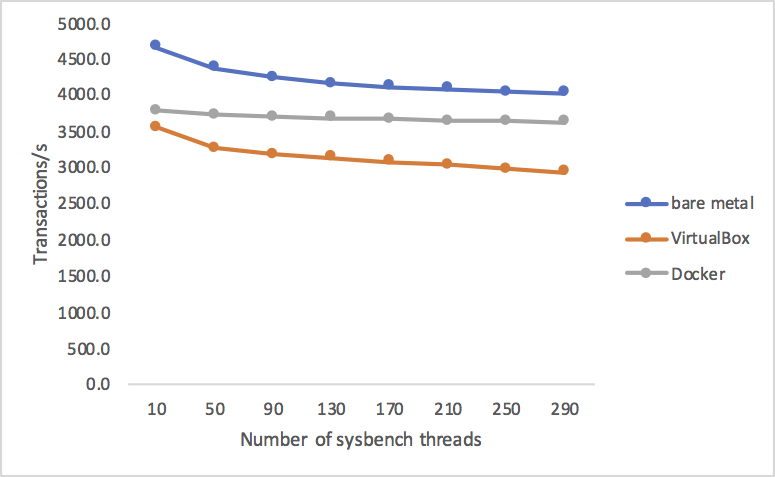
\includegraphics[scale=0.3]{mysql_throughput_graph.jpg}
\caption{Throughput results with MySQL when using the SysBench oltp benchmark with varying numbers of concurrent threads}
\end{figure}

\begin{figure}
\centering
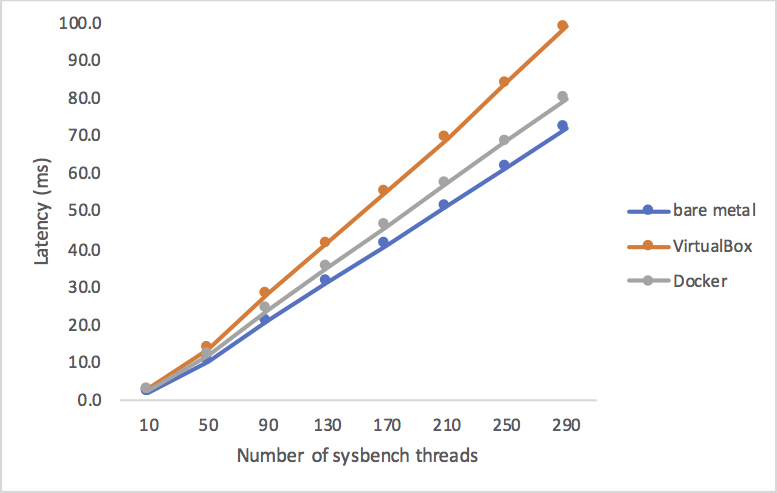
\includegraphics[scale=0.3]{mysql_latency_graph.jpg}
\caption{Latency results with MySQL when using the SysBench oltp benchmark with varying numbers of concurrent threads}
\end{figure}

\subsection{Discussion}
As the results show, the general trend of the benchmark results is consistent with those of the two papers. As expected, using VirtualBox, or any type of VM, introduces significant overhead compared to bare metal and containers. For almost all of the benchmarks and experiments, Docker exhibited very little overhead, which is consistent with the results shown by Felter et al. and Sharma et al. The one exception to this was the SysBench oltp benchmark when run on MySQL, where the performance difference between Docker and bare-metal was significant. This was likely due to different resource configurations. 

One surprising aspect was the magnitude of the overheads shown by the results for VirtualBox was surprising, as they were significantly larger than presented by both Felter et al. and Sharma et al. This is most likely due to the fact that VirtualBox is a Type 2 hypervisor, which introduces additional layers of abstraction over the hardware resources when compared to Type 1 hypervisors like KVM. KVM in particular is also capable of being tuned to improve performance in ways such as pinning vCPUs to physical CPUs. 

% --------------------------------------------------------------------------------------------- %

\section{Related Works}
As mentioned before, there is a sizable amount of literature on quantifying and evaluating the differences between containers and VMs. Besides for the two papers used to compare the results of this paper to, there are some other interesting and relevant studies as well. 

\textbf{High Availability:} Li et al.\cite{li:2015} approached the debate between containers and VMs from a different perspective from this paper, which was to examine their suitability for high availability when used for large platforms. They concluded that solutions already exist for VM or hypervisor-based platforms, the most common being failover clustering. However, extensions need to be made for container-based platforms as there is no mature feature for continuous monitoring, automatic failover and record-and-replay\cite{li:2015}.

\textbf{Edge Clouds:} Pahl et al.\cite{pahl:2015} also examined a different application of containers and VMs and discussed the application of containers and clusters for edge computing. Traditionally, one of the difficult aspects of edge computing with VMs is the migration of the image as it is quite large. Pahl et al. conclude that containers could potentially advance PaaS (Platform as a Service) technology towards distributed heterogeneous clouds because of their lightweightness and interoperability\cite{pahl:2015}. However, improvements still need to be made to deal with data and network management, as well as orchestration for clusters.

\textbf{Other Performance Comparisons:} Both Morabito et al.\cite{morabito:2015} and Joy\cite{joy:2015} also conducted performance comparisons of containers and VMs similar to those of this paper. Morabito et al. focused specifically on CPU, memory and disk I/O while Joy also examined the scalability aspect as well. Morabito et al. conclude that VM technology has improved drastically in terms of performance but disk I/O is still an issue, and also that containers have negligible overhead at the cost of isolation and security\cite{morabito:2015}. Joy concludes that containers outperform VMs in terms of both performance and scalability but VMs can still be more suitable depending on the use case. 

% --------------------------------------------------------------------------------------------- %

\section{Conclusions and Future Work}
Both containers and VMs are mature enough technologies now to warrant their prominence. Their clearly different approaches and implementations are manifested in the differences in performance results and use cases. The results from the benchmarks ran show that the general conclusions from the two papers are still consistent, though the magnitude of the differences is noticeably different in some cases. In general, Docker's performance equaled or exceeded that of VirtualBox, and also equaled that of the bare metal server. 

Along the course of this paper, there were a few noteworthy lessons learned and discoveries. The main lesson was around the complexity of not only the implementations of these virtualization options, but also the effective usage of them. Even with useful tools targeted to simplifying the use of virtualized environments like Vagrant, achieving the desired configuration was non-trivial. Furthermore, there exists a tradeoff between using tools like Vagrant and having fine-grained control over their configuration. In addition, to recreate some of the results for Docker's performance as shown by Felter et al. and Sharma et al., there was a large amount of parameter tuning for both the container and the benchmark configuration. This goes to show the importance of understanding the proper usage of these tools to achieve the best results.

An interesting area of future work would be to generate quantitative evidence for the claims discussed in the previous paragraph. This would involve running multiple virtualized environments simultaneously to benchmark both the effects of overcommitting for VMs and the effects of performance interference. Building off of this, a configuration could be developed to allow for containers to deploy inside VMs as effectively as possible. Similar benchmarks would be run on this as well to see the validity of this architecture.


% --------------------------------------------------------------------------------------------- %

%
% The following two commands are all you need in the
% initial runs of your .tex file to
% produce the bibliography for the citations in your paper.
\bibliographystyle{abbrv}
\bibliography{GP_bibliography}
\end{document}
